%\addcontentsline{toc}{chapter}{Kapitel-1}
\chapter{Partikel Erkennung}

In diesem  Abschnitt werden einige Möglichkeiten zur Erkennung von Partikeln in einem Video niedriger Auflösungsqualität verglichen und hervorgehoben. Es wäre natürlich ideal einen Vergleich zwischen manuellen und werkzeugbasierten Erkennung zu ziehen. Aber leider wird die manuelle Erkennung hier nicht vollzogen aufgrund der viel zu schwierig bzw. langwierige Arbeit, die es bereitet. Es geht hier nämlich um mehrere hunderte von Partikeln pro Bild. 
\todo{ ToDo: Ein Bild soll hier als Beispiel verwiesen werden.}
\\

In diesem Sinne widmet sich die Arbeit in der Folgezeit dem Vergleich möglicher Werkzeugen, die zur Erreichung der eigentlichen Ziele nutzen können. Hierbei werden aus der Vielzahl der Instrumente nur vier oder fünf herausgegriffen. Diese werden zunächst einer tabellarischen Grobanalyse der Merkmale und dann einer textuellen Analyse der Unterschiede unter ihnen unterzogen. \\

\todo{ ToDo: Zwei weitere Partikel-Tracking-Bibliotheken finden.}
\todo{ ToDo: Eigenschaften jeglicher Tool im Vergleich Anderer zu herausfinden}

\begin{tabular}{|c||c|c|l|}
\hline
Werkzeug & Schwerpunkt & Zugänglichkeit & Parameteranzahl \\
\hline
\hline
 TrackPy & & & \\
 \hline
 PyPIV   & & & \\
 \hline
 OpenPTV & & & \\
 \hline
 ??????  & & & \\
 \hline
 ??????  & & & \\
 \hline
\end{tabular}




%\addcontentsline{toc}{section}{Kapitel-1}
\section{Werkzeugbasierte Erkennung}

\subsection{Trackpy}
Trackpy ist ein Python-Paket, das es ermöglicht aus einem Video bzw. einer Imagesequenz Partikel in unterschiedlichen Dimensionen (2D und 3D) zu erkennen und zu verfolgen. Hier wird es natürlich die Zweidimensionalität anvisiert. Die Erkennung der Partikel erfolgt über eine der Funktionen des Paketes, nämlich die \textit{locate-}Funktion.
Dieser verfügt über eine reihe von Parametern, anhand derer die Qualität der Anerkennung ausgebessert werden kann.

	\subsubsection{Parameter der locate-Funktion}
		Folgende Parameter werden im Laufe dieser Arbeit angewandt:

		\begin{enumerate}
    			\item raw\_image: array \\
    			Wird für die endgültige Charakterisierung verwendet.
    			\item diameter: odd integer \\
    			Entspricht der geschätzten Größe der Partikeln (in Pixel).
    			\item minmass: float \\
    			Minimale eingebaute Helligkeit. Dies ist ein Schlüsselparameter, um störende 				Merkmale zu entfernen. Der Standardwert ist es 'None'.
%    			\item maxsize: float\\
%    			Maximaler Gyrationsradius der Helligkeit.
    			\item separation: float\\
    			Minimaler Abstand zwischen den Partikeln.    			
    			\item noise\_size: float or tuple\\
    			Breite des Gaußschen Unschärfekerns, in Pixeln. Der Standardwert ist 1.
    			\item topn: interger\\
    			Gibt lediglich die N hellsten Merkmale über minmass zurück. Wenn 							'None' (Voreinstellung), werden sämtliche Eigenschaften oberhalb von minmass 				zurückgegeben.
%    			\item preprocess: boolean\\
%    			Vorverarbeitung der Bandpass .
    			\item max\_iterations: interger\\
    			Maximale Anzahl der Schleifen zur Verfeinerung des Massenschwerpunkts, 					Standardwert 10.
%    			\item filter\_after: boolean\\
    			
		\end{enumerate}
		
Ein \textsc{Panda.Dataframe} mit den Daten \textit{y\-koordinaten, x\-koordinaten, mass, size, ecc, signal, raw\_mass, ep, frame} wird als Rückgabewert geworfen. Dies gilt für jedes der gefundenen Partikel.(Siehe )
Ausführlichere Informationen zu  weiteren Parametern sowie zu den Obengennanten ist auf zu ist.%~ \citep{Tp}% zu sehen. 
An dieser Stelle kann folgende Frage aufgeworfen werden: Was sind die besten Parameter? \\
Beachte, dass einfachheitshalber, während der gesamten Parametereinstellung nur das erste Bild unseres Videos betrachtet wird.

	\subsubsection{Welche sind die optimalen Parameterwerte für eine ideale Partikelerkennung?}
	Hier wird es ein Antwortversuch auf die zuletzt gestellte Frage eingegangen. Zur Erreichung dieses Zieles wird mit der Erkennung begonnen, indem nur die geforderten Parameter(raw\_image und diameter) verwendet werden und nach und nach weitere hinzugefügt werden, um die Suche zu verfeinern. 
	
	\begin{enumerate}
    			\item locate(f, d): Wobei f = raw\_image und d = diameter. \\ \\
    			 Während frames[0] entspricht in diesem Fall dem ersten Bild der Videoaufnahme bzw. der Imagesequenz. \texttt{frames} hingegen bilden die Gesamtheit der Bilder des Videos im Laufe der Zeit und damit die Sequenz der Bilder.  Diese Angabe, die vom Typ Array ist, stellt eine Voraussetzung für die Ausführung von Funktionen dar. \\
    			 Für den Durchmesser wird zunächst willkürlich eine ziemlich kleine ungerade Zahl genommen, um die Ergebnisse zu sehen und eine Annäherung an den Wert, den wir verwenden sollen, zu erhalten. Zunächst nehmen wir also einen Durchmesser von drei (d=3).  
    			 
\begin{figure}[H]
    \centering
    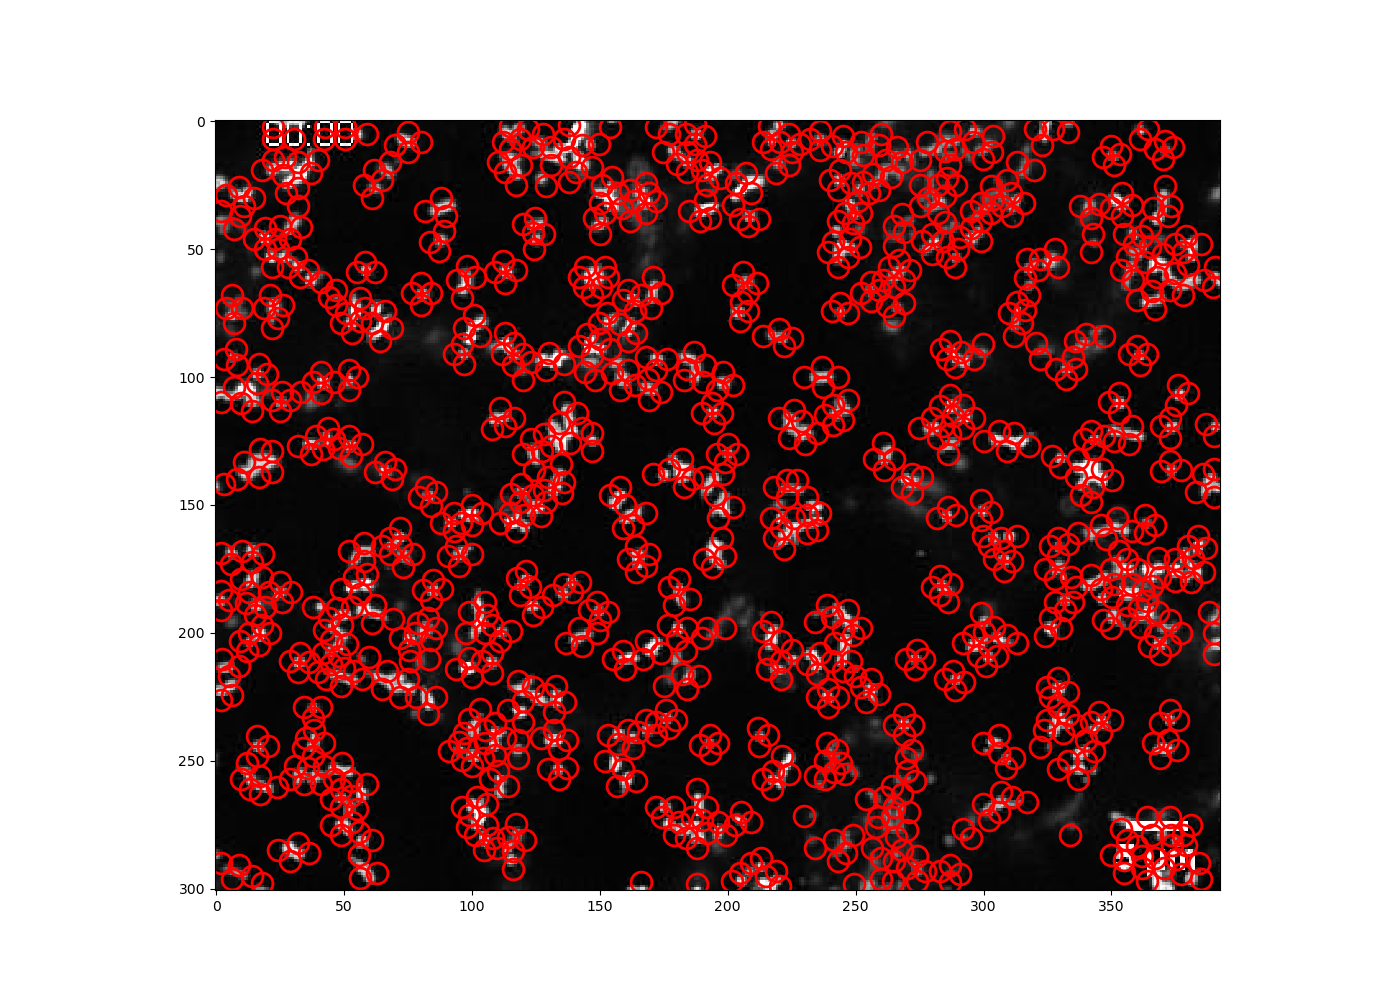
\includegraphics[scale=0.35]{Grafiken/trackpyBilder/locate(f0, diameter=3).png}
    \caption{locate(frames[0], 3)}
    \label{fig:bild_label}
\end{figure} 

Das Bild zeigt eine potente Lokalisierung der Partikel. Es wurde dabei fast alle Elemente des Bildes erkannt, wobei offensichtlich eine deutlich große Menge \textit{false Positive} ist. \\
Eine Verfeinerung der Lokalisierung würde somit einen größeren Durchmesser erfordern. Dies erfolgt in der Folge durch die Verwendung einer immer noch ungeraden Zahl, die jedoch einen größeren Wert hat. In diesem Fall ist es neun, da es so viele "False Positives" gibt. 
\texttt{locate(frames[0], 9)}

\begin{figure}[H]
    \centering
    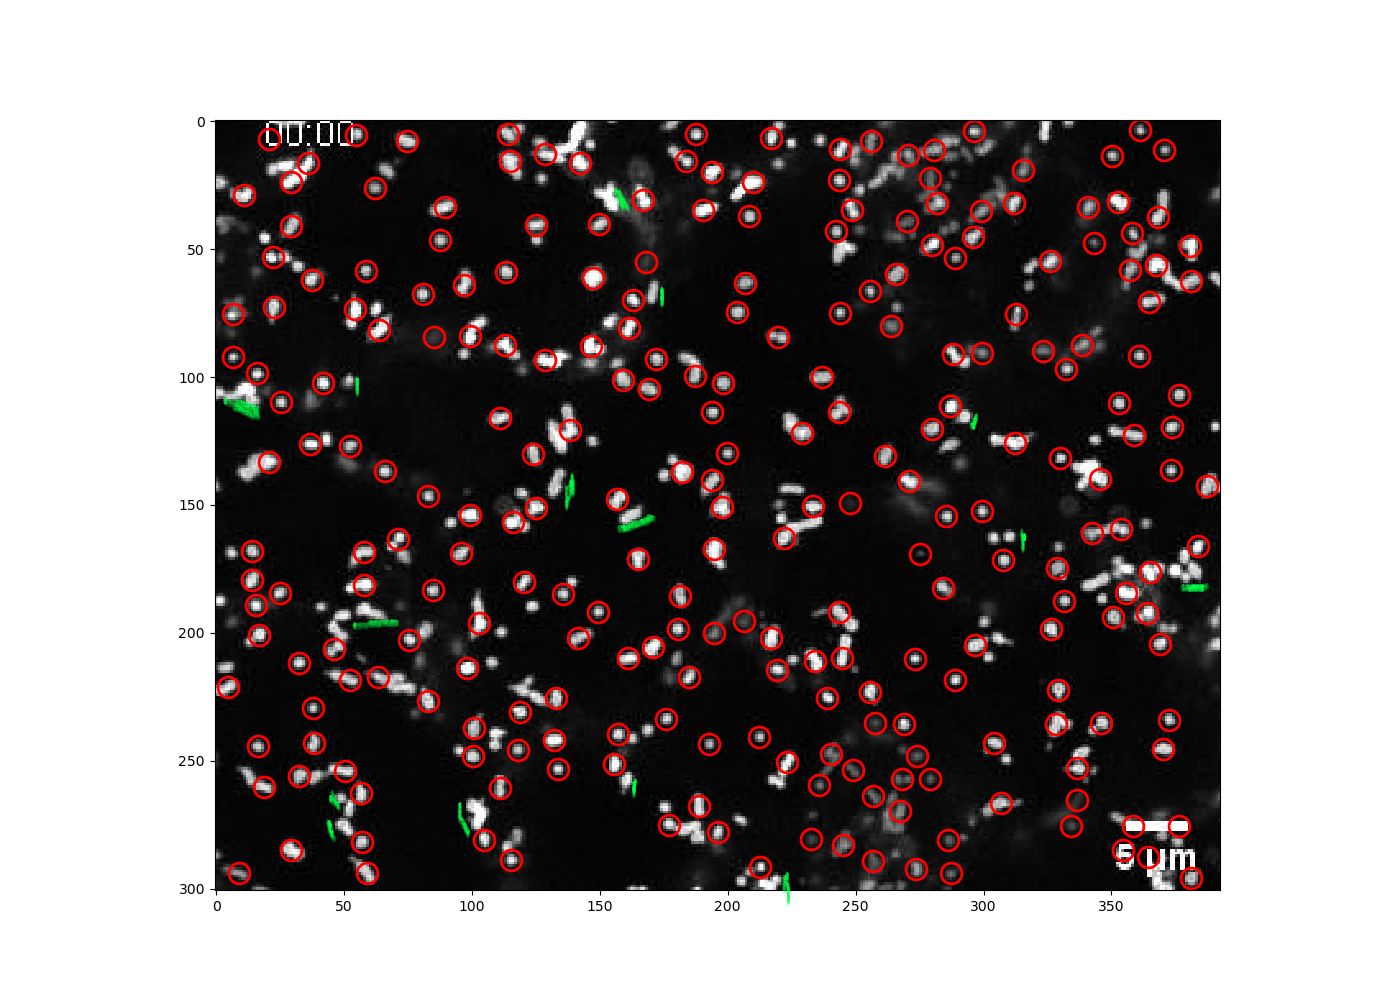
\includegraphics[scale=0.35]{Grafiken/trackpyBilder/locate(frames[0], 9).png}
    \caption{locate(frames[0], 9)}
    \label{fig:bild_label}
\end{figure} 

Diesmal gibt es zwar viel weniger ungewollte Teilchen. Allerdings hat sich eine große Anzahl von "False Negatives" gebildet. \\
Aus diesem Grund wurde nacheinander der Durchmesser von sieben und dann von fünf ausprobiert.\\
\texttt{locate(frames[0], 7)}   gefolgt  \texttt{locate(frames[0], 5)}
\newpage

\begin{figure}[H]
    \centering
    \begin{minipage}{.5\textwidth}
     	\centering
  	  	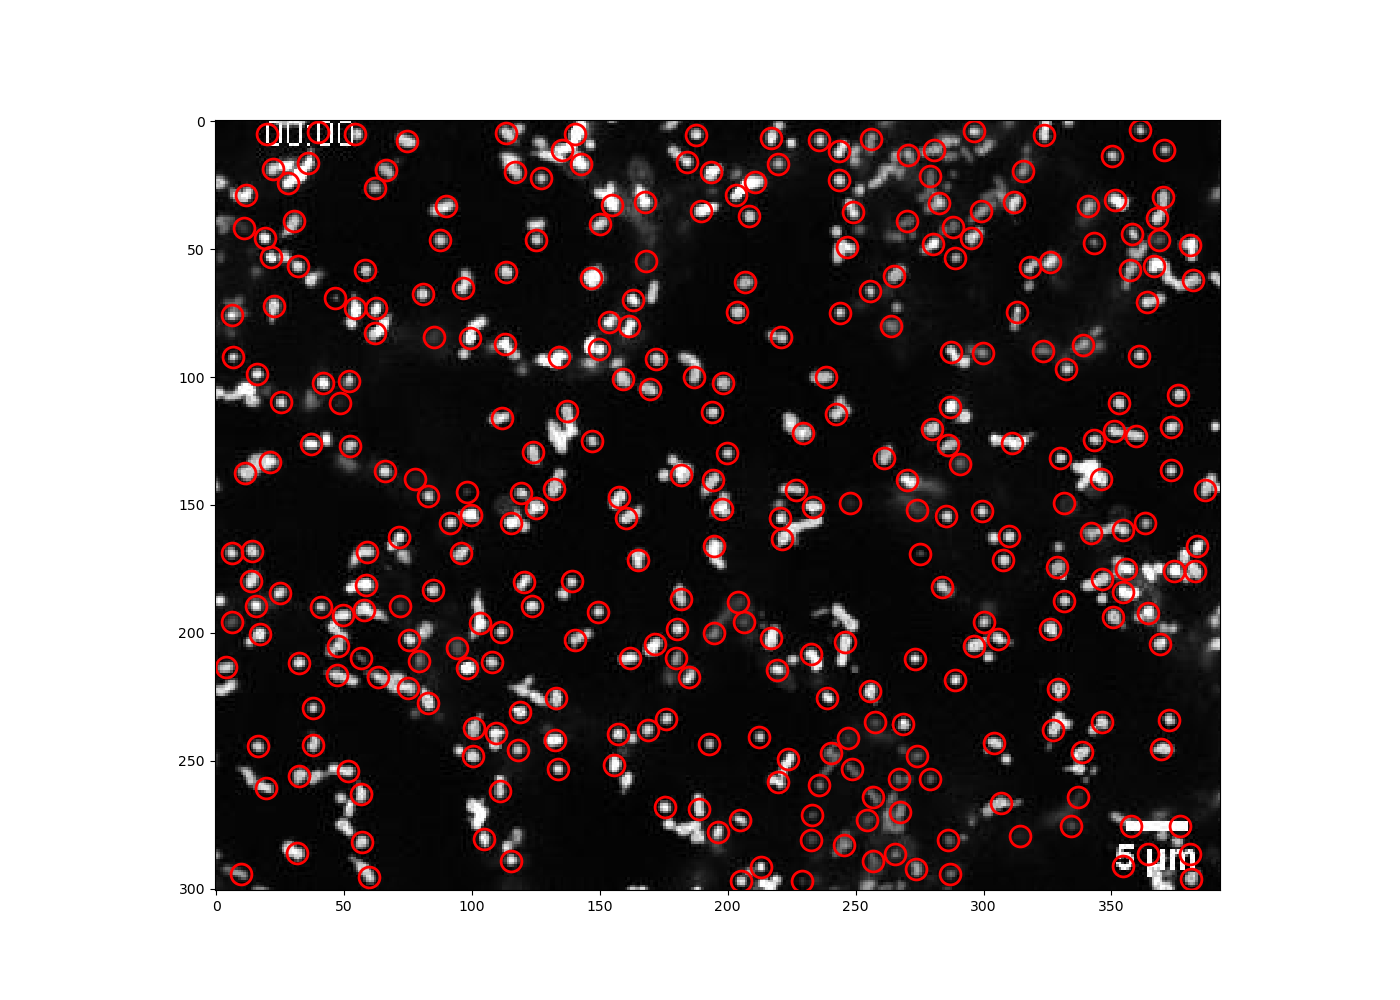
\includegraphics[scale=0.3]{Grafiken/trackpyBilder/locate(frames[0], 7).png}
 	 	\captionof{figure}{locate(frames[0], 7)}
 		\label{fig:test1}
    \end{minipage}
	
	\begin{minipage}{.5\textwidth}
     	\centering
  	  	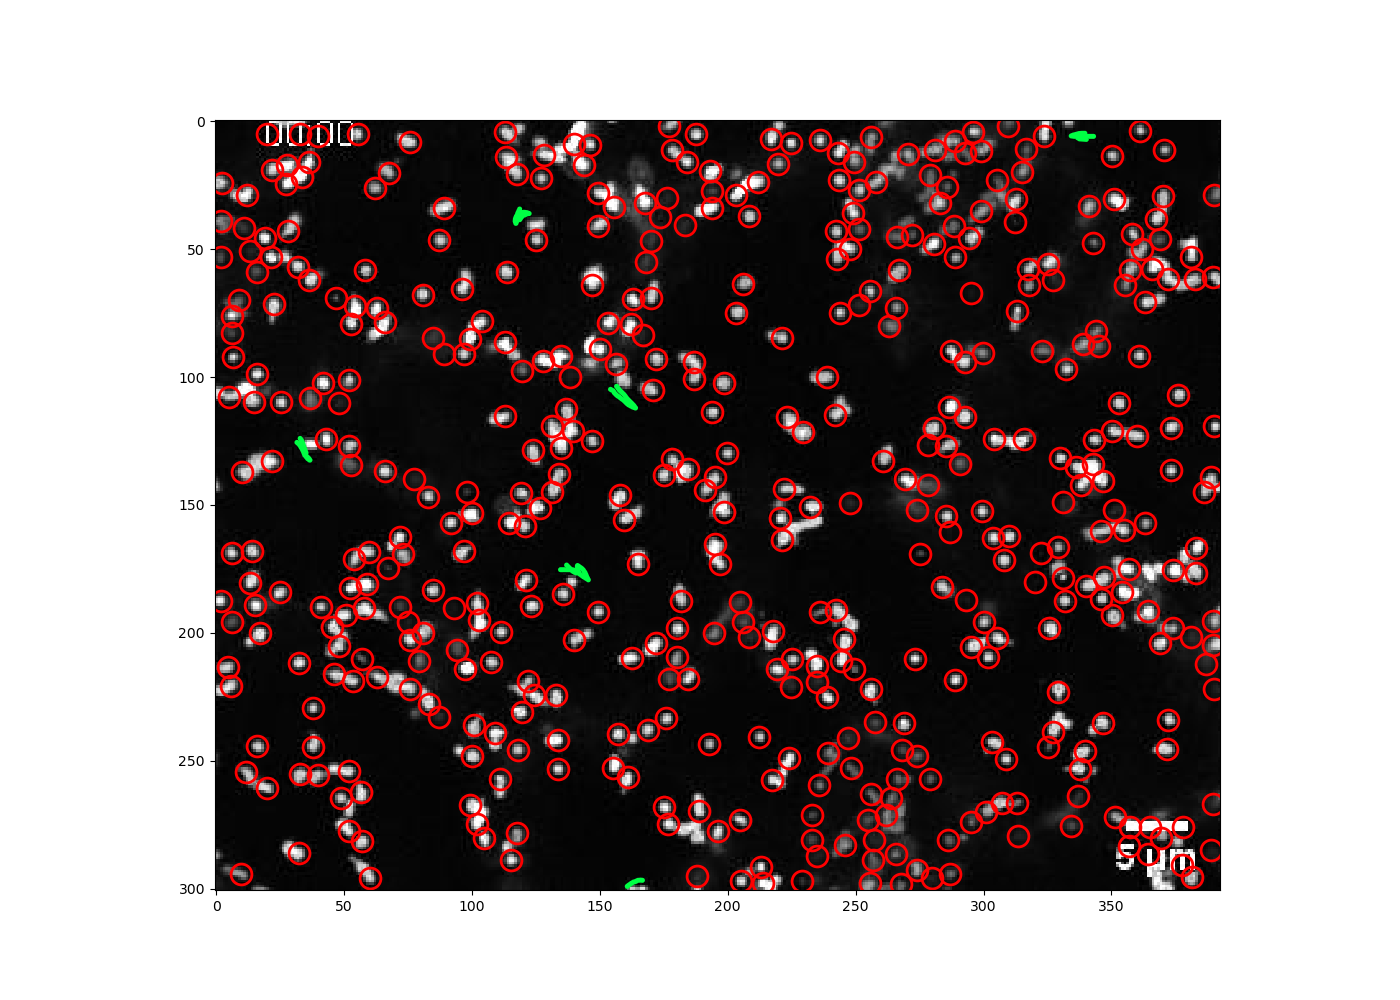
\includegraphics[scale=0.3]{Grafiken/trackpyBilder/locate(frames[0], 5).png}
 	 	\captionof{figure}{locate(frames[0],5)}
 		 \label{fig:test2}
    \end{minipage}
\end{figure}

In Anbetracht unseres Ziels, einen Durchmesser zu finden, der die Erkennung möglichst vieler Partikel ermöglicht und gleichzeitig möglichst wenig unerwünschte Partikel enthält, ist es besser, mit dem Durchmesser 5 fortzufahren. 

\begin{figure}[H]
    \centering
    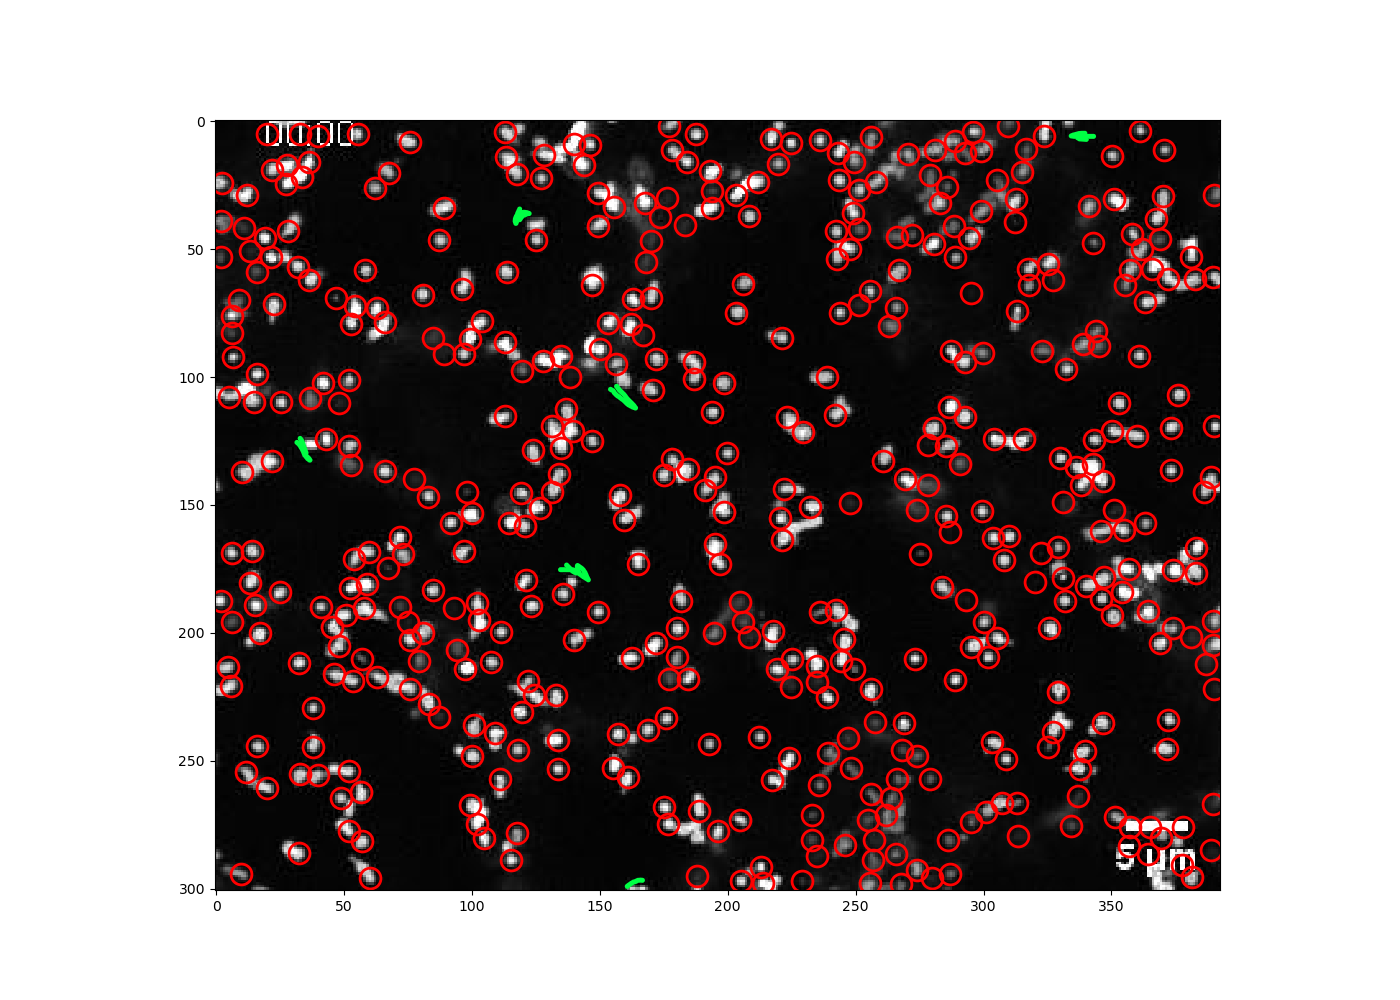
\includegraphics[scale=0.35]{Grafiken/trackpyBilder/locate(frames[0], 5).png}
    \caption{locate(frames[0], 5)}
    \label{fig:bild_label}
\end{figure} 
%    			 In diesem Sinne sieht das Ergebnis der Lokalisierung ohne weitere Parameter wie folgt aus:
%\begin{figure}[H]
%    \centering
%    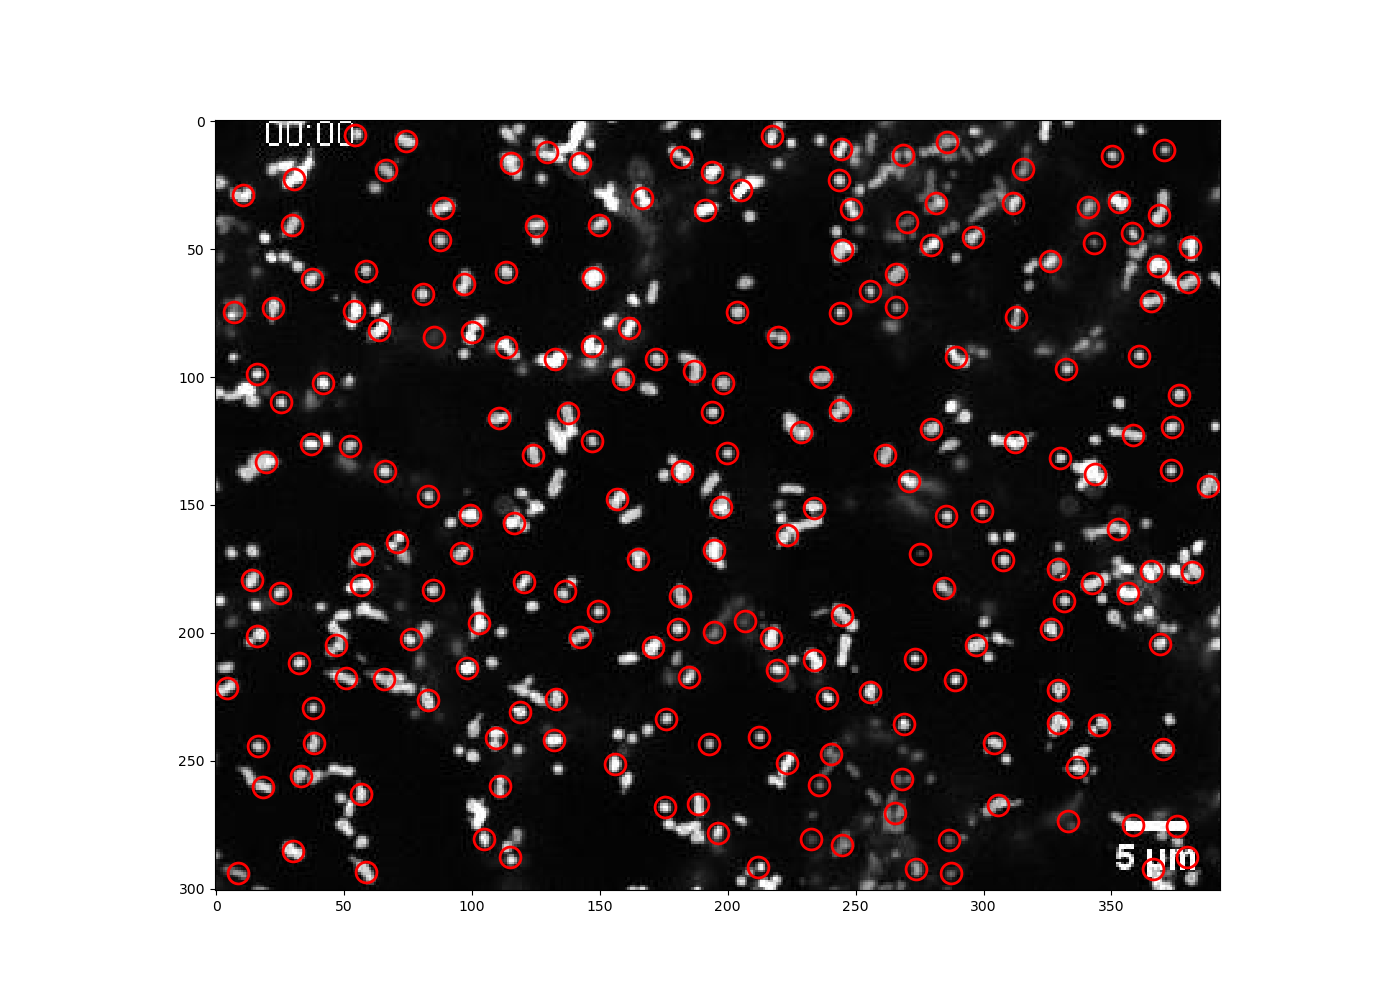
\includegraphics[scale=0.35]{Grafiken/trackpyBilder/locate_with_required_parameter.png}
%    \caption{locate with needed Parameters}
%    \label{fig:bild_label}
%\end{figure}
%    			Wie auf dem \ref{fig:bild_label} zu sehen ist, wurde eine Menge an Partikel 
%    			nicht erkannt, während andere unerwünschten erkannt wurden. 
%    			Insgesamt lassen sich 207 Partikeln finden, von denen 22 unerwünscht waren  und 91 fehlten. Dies entspricht einer ungefähren Rate von 10,628\% für die unerwünschten und einer Rate von 43,9617\% für die nicht gefundenen.

    			
    			\item locate(frames[0], 11, minmass=1000.0 ): \\ \\
    			Da ca. nur 10\% der letzten Suche unerwünschte Elemente waren, wird den Durchschnitt der \textit{minmass} aller Teilchen berechnet und als \textit{minmass} verwendet. Aus der vorherigen \textsc{Panda.Dataframe} genügt es den Mittelwert aus den Werten der \textit{mass}-Spalte zu berechnen, um auf \textit{minmass} von ca. 2490.21 zu gelangen. Das Resultat wird dann wie folgt aussehen:
\begin{figure}[H]
    \centering
    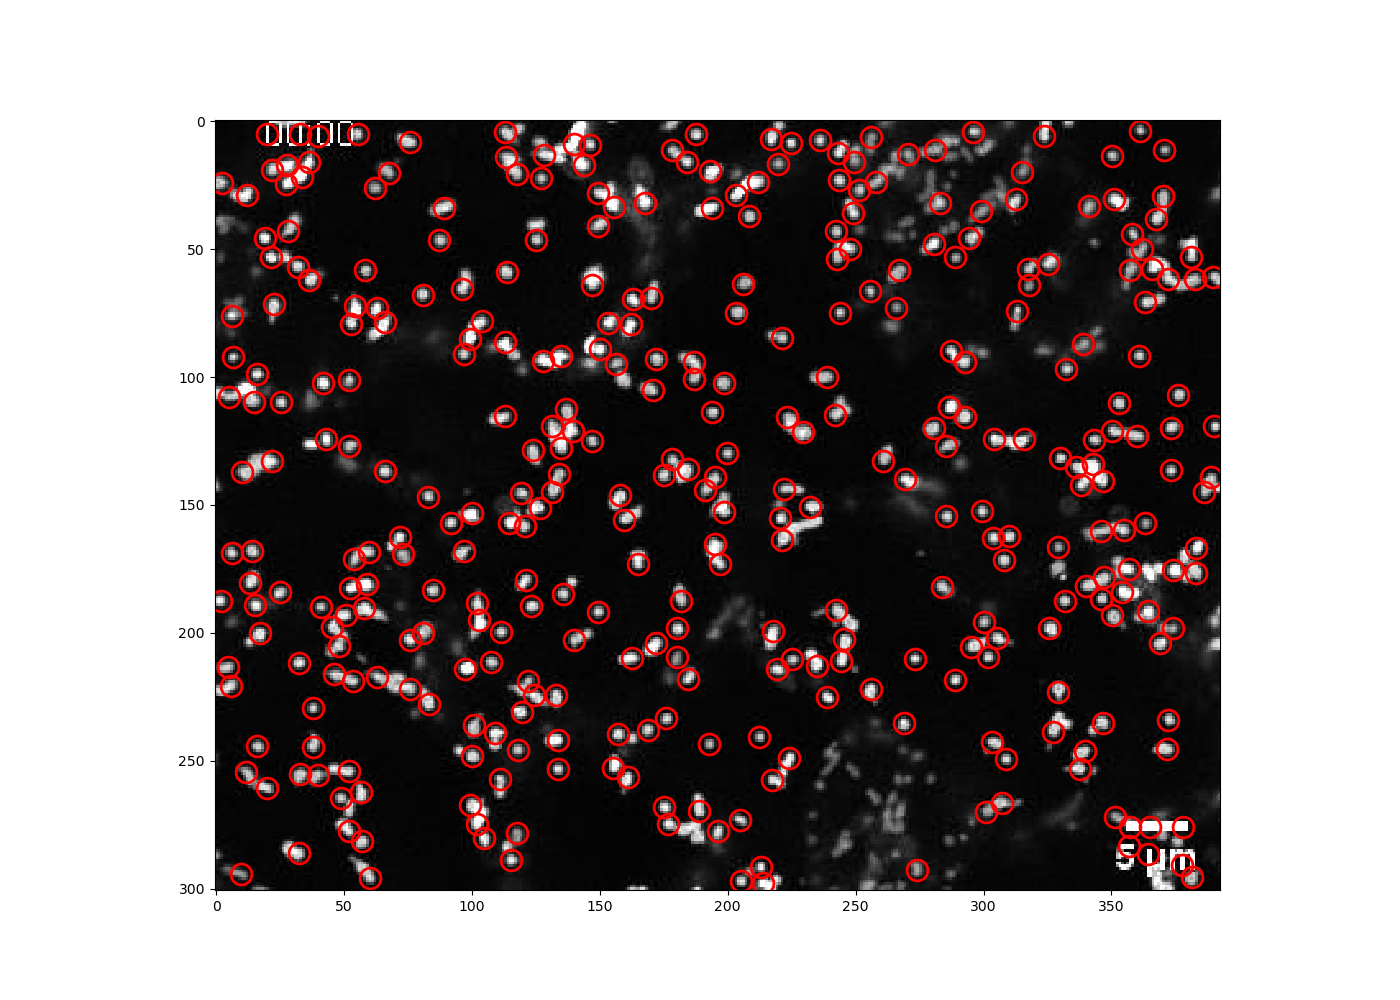
\includegraphics[scale=0.35]{Grafiken/trackpyBilder/locate_with_minmass_01.png}
    \caption{locate with 'mimass=2490,21'}
    %\label{fig:bild_label}
\end{figure}
Es wurde zwar fast alle \textit{False Positive} beseitigt, aber dafür wurde eine viel zu hohe Anzahl an \textit{True Negative} nicht gefunden. Die Lösung für dieses Problem besteht darin, den Wert von "minmass" schrittweise zu verringern, bis ein zufriedenstellenderes Ergebnis erzielt wird.
\begin{figure}[H]
    \centering
    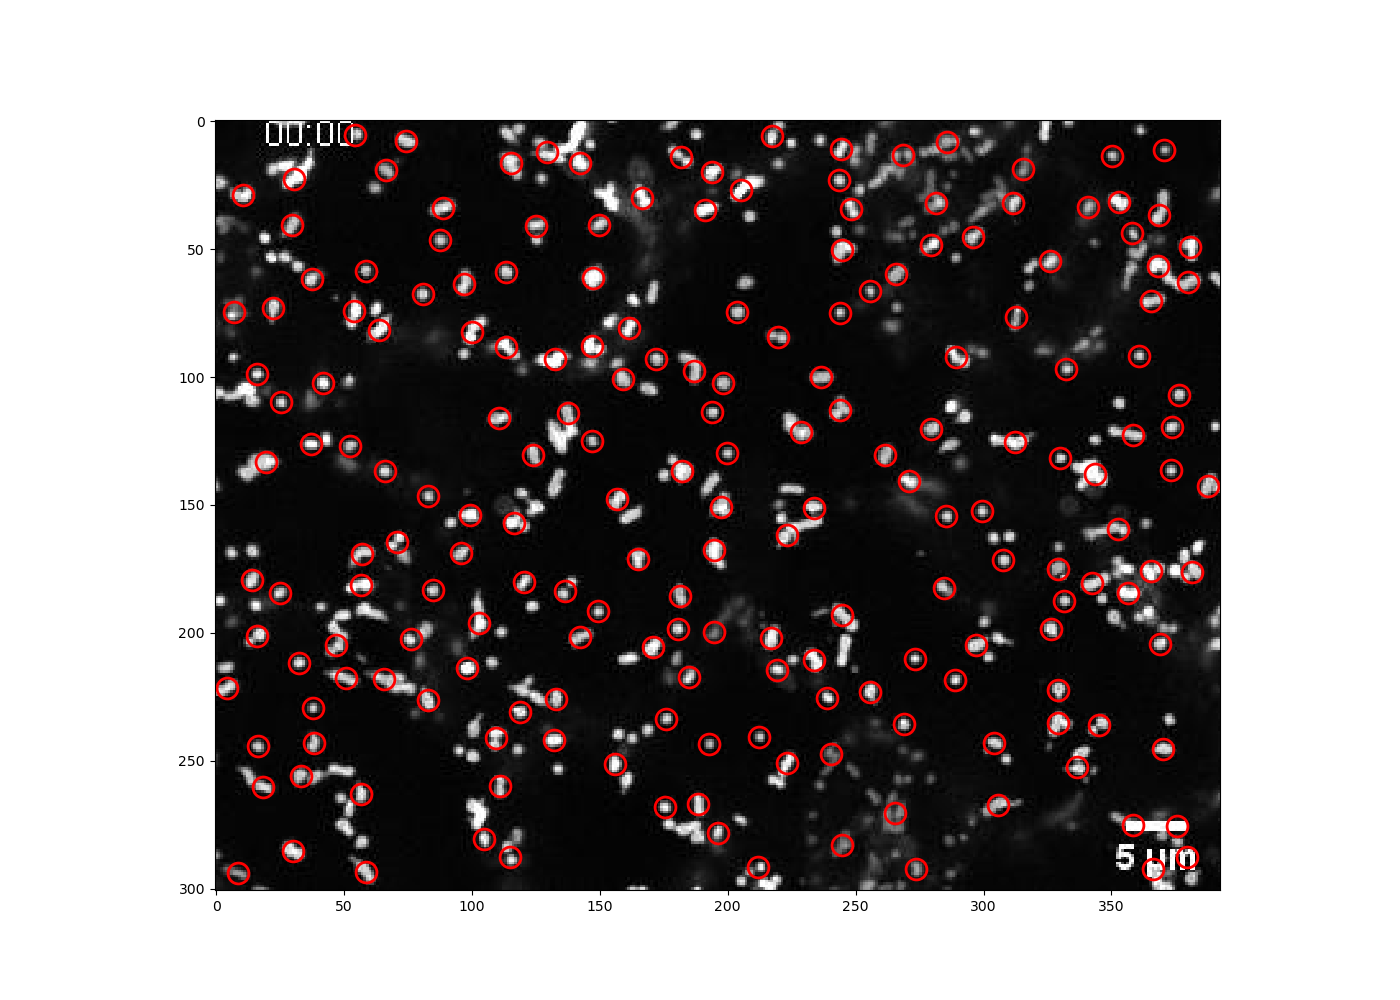
\includegraphics[scale=0.35]{Grafiken/trackpyBilder/locate_with_minmass_02.png}
    \caption{locate with 'mimass=1000'}
    %\label{fig:bild_label}
\end{figure}

		\item locate(frames[0], 11, minmass=1000.0, separation=2, noise\_size=1.5): \\ \\
    			Hier wird es einfach Werte bei \textit{separtion} und \textit{noise\_size} ausprobiert, um auf die bessere Resultate zu kommen. Dies ergibt in diesem Fall:
    			
\begin{figure}[H]
    \centering
    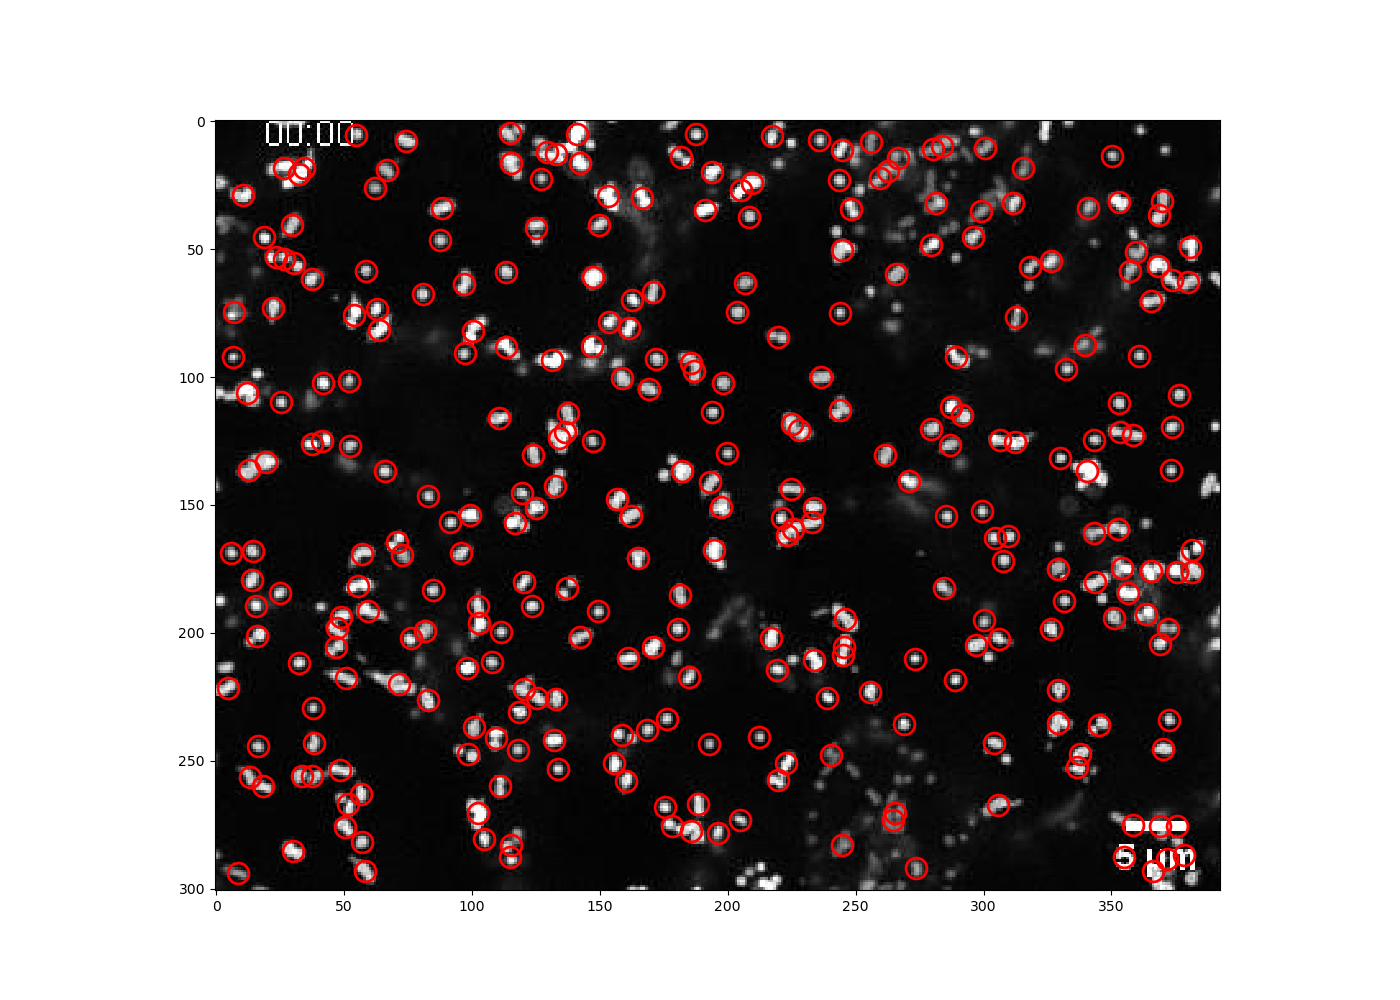
\includegraphics[scale=0.35]{Grafiken/trackpyBilder/locate_with_separation__noise_size.png}
    \caption{locate with 'sep=3.0 and n\_s=1.5'}
    %\label{fig:bild_label}
\end{figure}


\item locate(frames[0], 11, minmass=1000.0, separation=2, noise\_size=1.5, topn=250):    \\ \\ 
		Nachdem alle vorherige Parameter eingesetzt worden sind, wenn der Dataframe immer noch sanierungsbedürftig ist, wird auch \textit{topn} zum Einsatz gebracht. Dazu wird die Anzahl an bestehende unerwünschte Elemente geschätzt und von der gesamten Anzahl an gefundenen Elemente abgezogen. Somit wird \textit{topn} in dem Fall hier auf \textit{250} geschätzt. (siehe Bild)
\begin{figure}[H]
    \centering
    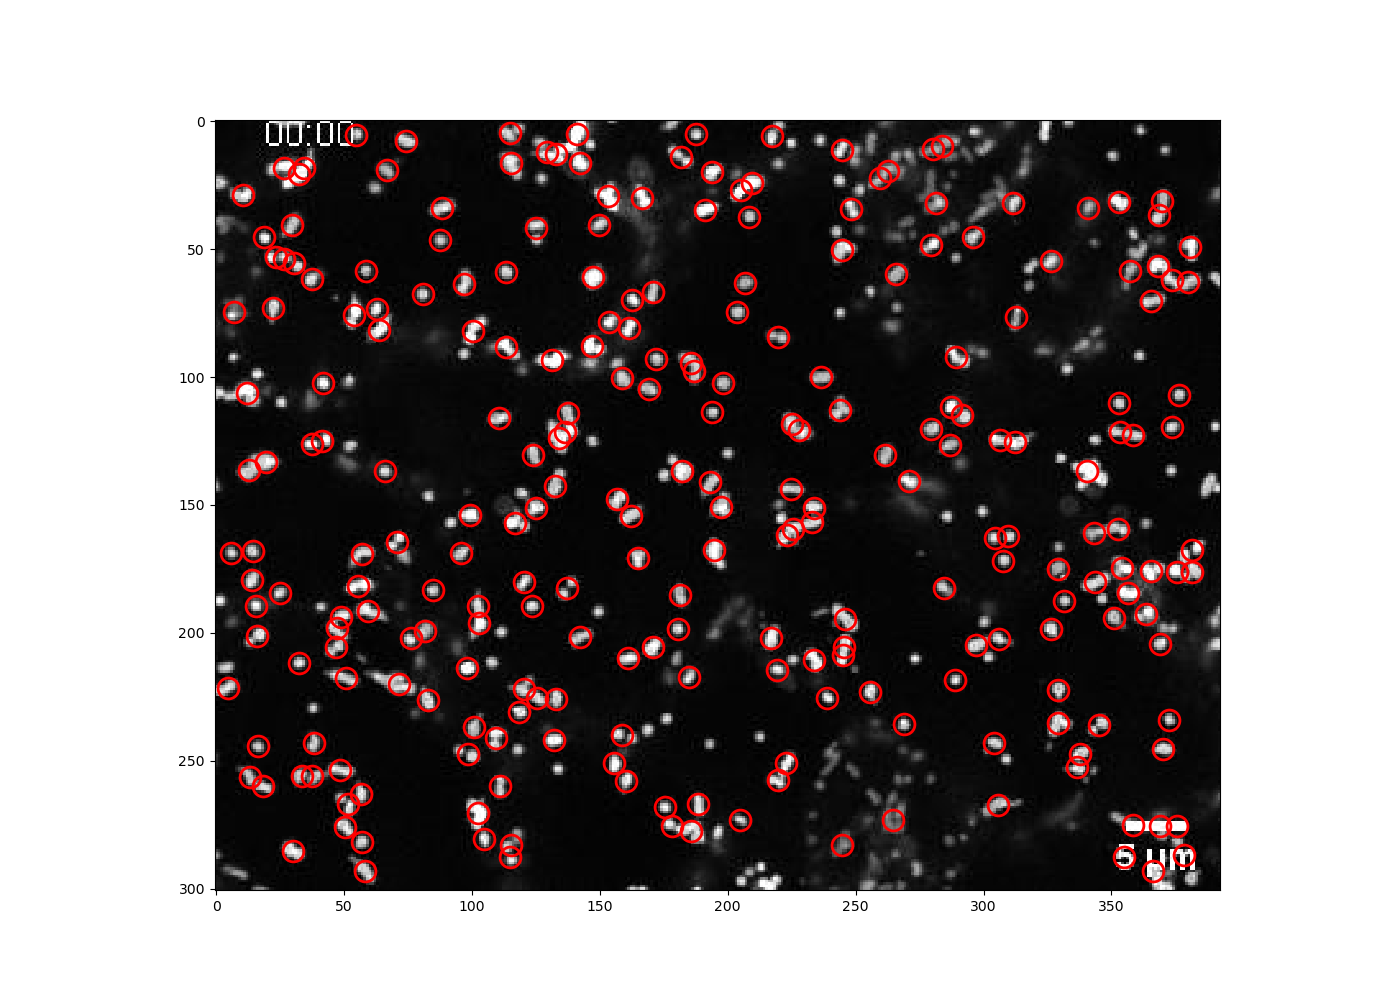
\includegraphics[scale=0.35]{Grafiken/trackpyBilder/locate_with_topn.png}
    \caption{locate with 'topn=250'}
    %\label{fig:bild_label}
\end{figure}
\end{enumerate}
\subsection{Machine Learning}


